\chapter{Theoretical Groundwork for Automated Parallel Methods}

\section{Motivation: Parallelism Necessitates Concurrency Control}
Consider that in the general case of a program intended for parallel execution,
the potential arises for two processors to perform computations that conflict
with each other. Specifically, when two processors access the same memory
location and at least one of them performs a write at that location, a conflict
arises, because both the code does not prescribe a global ordering of those
accesses and the order changes the outcome. Hence, this conflict results in a
program state that could potentially produce an incorrect result. Conflicts
occur when parallel programs cannot be mapped to unique sequential programs due
to their asynchronous properties -- at least one of the orders in which the
instructions could be executed, in combination with the program state, yields
an invalid program state at a later point in time.

In the most general case, it may prove challenging or impossible to prevent or
resolve these conflicts without relying on synchronization mechanisms that
prevent full utilization of parallel execution. But, if certain constraints are
applied to
\begin{enumerate}
    \item the operations that the processors will execute, and
    \item the read/write access patterns upon the data with which those
        operations will interact,
\end{enumerate}

the task becomes feasible. This in hand with a clever organization of memory
will yield automated parallelism methods.

\section{Groundwork for Minimal Concurency Control Mechanisms}
The following will assist in the description of concurrency control schemes that
come afterward.

\subsection{Terms, Definitions, and Assumptions}
We shall specify constraints for operations that processors may execute in
parallel in such a way that conflicts can be detected and eventually resolved.
These constraints give way to relaxations of the execution ordering of those
operations.

Each relaxation specifies a set of operations $\Op_{i}$ that contains all
functions that it allows. We assume that the operations have the form $\Op:
\mathbb{R}^{n} \mapsto \mathbb{R}$. If an operation effectively produces many
values, we model it as a series of operations that take the same inputs.  The
constraints will apply to the set $\Op$. The constraints may involve restricting
the domain to a subset of the general case above. In a practical setting, the
function's range will be the values allowed by a given numeric data type, such
as \texttt{uintXX}, \texttt{intXX}, or \texttt{float{XX}}, where $\texttt{XX}
\in {8, 16, 32, 64}$. We will refer to the inputs and output of a function as
\emph{values}, and in code, we will give them the general type \texttt{val}.

Then, we will provide a function $C_i$ which will identify a conflict, and a
function $R_i$ that will provide a way to resolve conflicts that arise.

Finally, we will define the set $St_{i,t}$ as the relevant subset of the program
state after $t$ operations. Here, relevant means that this program state works
in isolation with regard to all other operations taking place within the
program: no outside operations are reading or writing values in $St$;
furthermore, operations happening within $St$ do not read or write values
outside of $St$ either. Sometimes the program state is undefined for a certain
$t$, but we can place limitations on when this is acceptable \cite{timeclocks}.
Unless an operation produces no output, it modifies the program state via its
output.

\subsection{Caveats of parallelism}
For a task to incur speedup through parallelization, no overhead acquired
through managing parallelism must exceed the space or time complexity of the
serial version of the program. Call $\eta(\vec{x})$ the overhead of a given
parallel execution $f_p(\vec{x})$, with corresponding serial execution
$f_s(\vec{x})$. We then want
\begin{align*}
    \eta(\vec{x}) \in o(f_s(\vec{x}))
\end{align*}

in space and time. For example, a parallel algorithm for summing a set of values
should take $\Theta(\log(n))$ time assuming no overhead. An optimal serial
algorithm takes $\Theta(n)$ time -- no faster algorithm can exist. The overhead
to the parallel algorithm should take asymptotically $o(n)$ time or the
parallelization amounts to no asymptotic improvement.

Consider that any variable in a program has a set of dependencies. A dependency
is another variable used to compute the first's value at some point during the
computation. Adjacent dependencies appear immediately in these computations, and
those may have their own dependencies as well. Construct a dependency graph $G$
for a variable in a subroutine. The graph begins as a single node, just the
variable itself; call it $v_0$. Iterate through the execution paths of the
program until the variable receives an assignment of some value. If the value is
constant and does not come from the evaluation of an expression, do not modify
the graph. If the value comes from the result of an expression, take each
variable inside the expression and add them to the graph, drawing a directed
edge from each of them to $v_0$. Continue doing this until $v_0$ shares an edge
with every variable contained in an expression assigned to $v_0$. Then, repeat
the process for each of these newfound dependencies. If the assignment to $v_0$
results from a function call, then this process must be repeated with the return
value of the function in question, which itself serves as the sole direct
dependency of $v_0$ from the call. Note that the graph may have cycles. In fact,
very simple subroutines have cycles. For example, incrementing a counter has one
node and an edge connected to itself -- a loop. Now, take any paths for which
each node in the path has only a single incoming and outgoing edge and compress
them into a single node. These paths result from inherently serial computations.
The number of intermediate variables used to represent these computations is
incidental and nonessential to the graph's meaning. Such subgraphs cannot be
parallelized, as each operation depends exactly on the preceding one. As an
example, computing $\sin(\log(x))$ requires performing $\log(x)$ and then
computing the $\sin$ of the result. The logarithm must be computed first. Having
two processors at hand cannot speed up this computation.

The longest path that doesn't repeat a node serves as a lower bound for the
runtime of the subroutine as each edge has at least $O(1)$ time complexity. A
tighter lower bound would come from determining the complexity of the number
of times each cycle in the graph would be performed and to identify the longest
path with repeated edges, bounding the number of times a node is incorported to
the unique cycles that contain it. Then, each of those cycles would contribute
its complexity to the lower bound of the complexity of the runtime of the
overall subroutine.

Consider a partition of the edges of the compressed graph by its connected
subgraphs. These subgraphs can be executed independently, yielding parallelism.
Now consider removing an arbitrary node $n$ from the graph. If the number of
subgraphs increases due to the removal of $n$, then the newly-generated
subgraphs correspond to sections of the subroutine that are computationally
independent. Without loss of generality, say there are 2 such newly-generated
subgraphs $P$ and $Q$. There are three cases for how these subgraphs $P$ and $Q$
interact:
\begin{enumerate}
    \item All edges $e \in E(P)$ incident to $n$ are \textbf{incoming} to $n$,
        and all edges $e \in E(Q)$ indicent to $n$ are \textbf{outgoing} from
        $n$: $n$ connects $P$ to $Q$, and $Q$ can only be computed once $P$ has
        been.
    \item All edges $e \in E(P)$ incident to $n$ are \textbf{incoming} to $n$,
        and all edges $e \in E(Q)$ indicent to $n$ are \textbf{incoming} to $n$:
        $P$ and $Q$ can be computed in parallel, but the value of $n$ can only
        be determineded once both $P$ and $Q$ have been computed.
    \item All edges $e \in E(P)$ incident to $n$ are \textbf{outgoing} from $n$,
        and all edges $e \in E(Q)$ indicent to $n$ are \textbf{outgoing} from
        $n$: $P$ and $Q$ can be computed in parallel, but only once the value of
        $n$ has been determined.
\end{enumerate}

In the latter two cases, opportunities for parallelism exist, and $n$ identifies
a point where concurrency control must take place to ensure the correctness of
the program. In (2), $n$ identifies the point at which synchronization between
the two parallel regions $P$ and $Q$ must occur: $n$ must wait for both to
finish before issuing the expression to which it corresponds, because it depends
on the result of those independent computations. In (3), $n$ identifies the
point at which parallelism can begin.

Ultimately, this partition results from cuts of the graph along these edges. In
(1), two such cuts are required to separate the subgraphs from $n$. The cut
indicates that $n$ has a read dependency on $P$ -- it must read the value that
subgraph produces at the node opposite the cut edge in order to perform its own
computation. Furthermore, $Q$ has a read dependency on $n$, and cannot begin its
execution until the value of $n$ has been determined. In (2) and (3), only one
cut is required, as there are no dependencies between P and Q themselves, and
the cut can separate both P and Q into the same region apart from $n$.

At some point, execution of each subgraph must take place. It can either take
place eagerly, as soon as the program begins running, lazily, exactly when some
node depends on it and only it, or somewhere in-between, such as at some
position in an arbitrary or reasoned execution ordering given by the programmer
via language semantics, compiler, interpreter, or runtime. If a task computes
eagerly and before necessary, it may take up processor time better used
elsewhere, causing other, more critical procesesses to wait for it. If a task
computes lazily and inopportunely late, other tasks that may depend on it may
have to wait as well. Schedulers cannot always account for these dependencies,
resulting in idle processors and synchronization overhead.

\subsection{Commutative and Associative Operations Allow Dependency Relaxation}
These graphs may prove too rigid when trying to achieve maximal levels of
parallelism in a program. Some apparent dependencies in the graph, as
constructed above, may not actutally hold with regard to program correctness.
Consider, for example, a case where a processor performs multiple additions on
some value, and that all other addends of those additions are determined by
mutually independent subgraphs. The graph produced above may look like a stick
with one additional incoming edge at each node; each node in this subgraph then
has two incoming edges and one outgoing edge, because the additional incoming
edge at each node connects other independent subgraphs. But, the order in which
these additions take place does not affect the final outcome. The following
explains a more general method for identifying these situations and allowing
more parallelism to take place in light of them.

We can limit our set of operations to commutative, associative reductions.
This is such that:
\begin{align}
    & \Op_0 = \left\{f\right\}  \\
    & f: \mathbb{R}^2 \mapsto \mathbb{R}  \\
    & f(x,y) = f(y,x)  \\
    & f(x,f(y,z)) = f(f(x,y),z) 
\end{align}

The result is that if you have a set of values $V$ and would like to apply $f$
onto $V$ repeatedly, you can do so by selecting arbitrary $x \in V$, and
performing $V = \left\{ f(x,y) \cup V \setminus \left\{ x, y \right\}
\right\}$.  This implies that our desired start and end program states are:
\begin{align*}
    St_{i,0} &= \left\{ V \right\}  \\
    St_{i,T} &= \left\{ v_\text{ans} \right\}
\end{align*}
where $v_\text{ans}$ is the single value resulting from performing the reduction
of $V$ as described above.

In pseudocode, each task might appear as follows:
\begin{lstlisting}
/* preconditions: 
    - reduce is only called if size(V) > 1
    - remove() and add() are atomic upon the set */
void reduce(set<val> &V) {
    val x = V.remove();
    val y = V.remove();
    ans = f(x, y);
    V.add(ans);
}
\end{lstlisting}

Notice that the operations on $V$ must be atomic because the function mutates
it.  Thus, \texttt{reduce} has side effects, and the operations upon it must
preserve atomicity lest two processors, e.g., try to remove the same element.
Similarly, we want to avoid adding an element to a set in such a way that
disrupts other processors' actions upon that set.

The implementation of this reduction on a shared or distributed memory computer
remains unspecified; a shared memory implementation will be provided in section
\ref{explain:indexmaps}. One can envision more or less efficient versions with
different pros and cons. For example, using other concurrency control
techniques, contention can be reduced. A natural direction, described in more
detail in \ref{explain:indexmaps}, involves giving processors ownership over
mutually exclusive subsets of values in $V$, having them perform reduce
operations on only the values they own, and then using the above strategy to
arrive at the final value only when each processor has exactly one value left.
Essentially, delegation of values does not have to happen through the atomic
removal of arbitrary values from the set, though doing it this way allows us to
describe an arbitrarily ordered method for performing such reductions without
any extra machinery or complexity. Conveniently, it also has the side effect of
load-balancing the parallel computation, because each processor stays busy until
\texttt{size(V) == 1}, or one step away from the end of the subroutine.

One might ask, why not design the reduction as follows:
\begin{lstlisting}
/* preconditions: 
    - reduce is only called if !isempty(V)
    - remove() is atomic upon the set */
void reduce(set<val> &V, val &ans) {
    val x = V.remove();
    ans = f(ans, x);
}
\end{lstlisting}

The answer is simple: the entire second line of the function must be atomic,
because if another processor modifies \texttt{ans} after it is accessed and
before it is assigned, the intermittent update to \texttt{ans} has been erased.
Because the entire second line must be atomic, no parallelism occurs.
Implementing the code in this manner results in no parallel speedup. The
executions of $f$ must be able to occur on multiple processors simultaneously:
this is the definition of parallelism, after all. But, leveraging persistent and
transient structures will allow us to achieve code along these lines without
needing such atomicity or synchronization while still yielding the correct
result.

\subsection{Persistence and Mitigating Synchronization}
A persistent data structure is a data structure that appears immutable from all
references. That means that any data accessed through a particular variable
stays the same, no matter when you access it and no matter what other
operations you supposedly perform on that data structure, i.e., any functions
you call that involve that data structure. Object-oriented languages would frame
the data structure as a class with member functions; others would frame the data
structure as a composite type with corresponding functions that accept it as
an argument and mutate it. Data strutures in purely functional languages would
operate like persistent data structures but with additional strictness: the data
structure does not only appear immutable from all references, it \textit{is}
immutable from all references, and the proxy for mutation involves producing a
new data structure that corresponds to how the original one would look after the
desired mutation.

Define a transient data structure as a data structure that behaves as the above
one in all cases except through two documented functions: \texttt{resolve} and
\texttt{deregister}. The first, \texttt{resolve}, updates the data structure to
correspond to the most recent version of it, incorporating changes across all
processes. This will take some amount of time. Next,
\texttt{eregister} tells the underlying data structure that the elements
referred to need not stay accessible any longer. It allows the data structure to
clean up old values that no longer have any use for the program. In a persistent
setting, the same mechanism takes place when the variable falls out of scope.
But, sometimes, optimizations can be made that would be cumbersome using only
this construct. Highly-nested code blocks that delineate the lifetime of
variables should not serve as the only means of writing efficient programs using
persistent data structures, and furthermore, an efficient program may require
the resolution of a transient data structure after versions of it have already
fallen out of scope, require the extension of the lifetime of those other
versions.

\newcommand{\toper}{t_\mathrm{oper}}
\newcommand{\tcomm}{t_\mathrm{comm}}
\newcommand{\tpar}{t_\mathrm{par}}
\newcommand{\tser}{t_\mathrm{ser}}

In this work, we develop CT (Contended Transient) data structures that add
reconcilability to simultaneous modification. When two processes modify a
variable at the same logical time, then necessarily, neither process can see the
desired final value of that variable without more work. In a lock-based setting,
the extra work would involve two locks and two unlocks. In a persistent setting,
the extra work would involve the creation of two extra variables and one extra
addition. Those variable creations can be pre-allocated in settings where
conflicts are likely, resulting in an overhead of just one extra addition. But
in the case of a very small number of additions, the benefits of parallelization
don't manifest -- one processor can handle such sequences of operations best,
negating any synchronization costs.

Then, if other distributed processors need the data, an immediate or queued
message can be sent to them by some prioritization. But, if many additions are
performed, or if complex sets of operations are performed, a method for
parallelizing the tasks and reconciling the conflicts that arise, one optimized
for minimal overhead, becomes beneficial. Precisely speaking, parallelism
becomes beneficial once
\begin{align*}
    \eta + \tcomm \leq \tser \text{,}
\end{align*}

where as before, $\eta$ describes the runtime overhead of synchronization.

\section{Contention Resolution with CT Data Structures}

\subsection{Tools for Shared Memory}
Shared memory models allow many processors access to the same memory locations.
The latency of memory accesses are approximately the same among these
processors; simultaneous reads can be performed harmlessly. But, simultaneous
writes, or interleaved reads and writes, can lead to situations where different
processors perceive a conceputal value differently. In the case of the
aforementioned relaxation, problems arise when the list that contains the values
loses or gains elements, and certain processors tasked with performing the
reduce operation on certain values access the wrong values because they intend
to remove certain values from the list but instead remove others. This case
arises when other processors have already removed those elements. Contention
only arises when processors use information affected by other processors: If
there are $N$ values to reduce and $P$ processors, then as long as $P \leq N/2$,
then each processor can perform at least one operation for which no contention
exists. Each processor has two values that it can reduce independent of all
other processors. Otherwise, any processor must use data that another processor
has produced, or may try to use itself, and barring algorithmic strategies
designed to handle contention (i.e. synchronization), processors will interfere
with each other. Even under such strategies, processors may need to wait idly
for the algorithm to allow them to continue safely or may end up doing
unnecessary work to arrive at the correct answer.

From the perspective of organizing all necessary reduce operations, different
strategies exist, and the traditional notion of contention that arises in this
laissez-faire understanding of shared-memory parallelism accepts many
categorically different strategies.

\subsection{Preemptive Contention Resolution}
Preemption can resolve the contention issues above. For example, consider that
each processor has an ID and can compute the set of indices in the original list
that it can be said to \emph{own}, such that any computation involving values
that it owns. In the case where $2P \leq N$, then we can say each processor owns
values $e_i$ for $P \leq i < P + \ceil*{\frac{N}{P}}$, which allows each
processor to own a contiguous block of values that it can perform the reduce
operation independent of the other processors. When $2P > N$, then we can say
that for two processors $p_i$ and $p_j$ where $i < j$, if a reduction must be
done upon a pair of values owned, respectively, by each processor, $p_i$ will
perform the reduction. At this point, each processor owns at most one value, so
this strategy incurs no wasted cycles due to idle processors. Note that
processors with larger IDs may now spend their time on other tasks, such as
other computations without interprocessor dependencies, or in a distributed
memory setting, the asynchronous communication of already-computed values on
which other processors depend.

Preemption incurs an overhead: each processor must know its ID, and as soon as
$2P > N/2$, a comparison must execute to determine which processor will handle
the following reductions. Ultimately, the overhead here is constant in the number
of values to reduce and logarithmic in the number of processors ($O(\log_2 P)$
extra comparisons). Furthermore, each processor in this final stage must receive
a signal that it can safely access the corresponding value it did not itself
compute: it must either block until the computing processor releases the final
value (using, for example, a mutex) or receive an explicit message (such as
through message passing, an actor, or a future) alerting it that it can use the
value. Essentially, an indeterminate amount of time might elapse before this
happens, approximately upper-bounded by the serial runtime of the program
including the overhead incurred through the synchronization infrastructure in
place (unless bugs produce deadlock, which would cause the program to hang
indefinitely).

\subsection{Postemptive Contention Resolution}
Postemption accounts for and corrects contention issues after they occur.
Postemption requires a formal understanding of the difference between expected
and observed results. A particular reduction corresponds to a detection function
that returns a boolean identifying whether contention resulted in an incorrect
interleaving of parallel operations. Then, a resolution function can attempt to
produce the correct value. Some resolution functions can themselves yield
answers identified as incorrect by the detection function, and some could
deterministically produce the correct result.

Say we have two processors $p$ and $q$. Processor $p$ has a dependency on value
$d_q$ to be computed by $q$ for its subgraph $G_p$, and processor $q$ has a
dependency $d_p$ to be computed by $p$ for its subgraph $G_q$.

In a postemptive scheme, if $q$ has always computed $d_q$ before $p$ accesses
it, then there could be potentially no concurrency control overhead. This
precludes any verification of the shared values -- it does not provide a
mechanism for determining if the value $p$ receives has, in fact, derived from
the expected computation by $q$. This leaves the desire for a scheme that
performs this verification with minimal overhead. Let's call this overhead
$\nu_\text{post}$. In the case where this value may depend on the uncertainty
inherent in parallel computation, we can discuss the expected value of this
term, $\Ev[\nu_\text{post}]$.

Say that the values $d_p, d_q$ are stored in a CT vector $v$ at indices $i_p$
and $i_q$ respectively. Treat the vector transiently when updating values that
do not serve as interprocessor dependencies (i.e., not $d_p$ and $d_q$), but
otherwise, perform persistent updates to its values. When it performs a
persistent update, it runs a routine that addresses the possible synchronization
problems. Consider the case of $p$ updating $d_p$ and that $d_q$ depends on
$d_p$. When $d_p$ is updated, its routine performs the following tasks:
\begin{enumerate}
    \item Update $q$'s reference to $v$;
    \item Run $C$ on $d_q$;
    \item If $C$ detects a conflict, run $R$ on $d_q$.
\end{enumerate}

At the point where $C$ is run, $d_q$ may have been updated using $f$, or not:
$p$ cannot know because no synchronization has taken place. $C$ will determine
if this is the case. $C$ has access to: (1) the version of $v$ that $q$ used
when it updated $d_q$, and hence that it used to access $d_p$, and (2) the fresh
version of $d_p$. It looks to see if $v[i_p]$ agrees with the fresh $d_p$. If it
does, it knows that the resolution is unnecessary. If it does not agree, then it
performs $R$ on $d_q$, using the defined resolution function $R$ for the
function $q$ ran to update $d_q$. This resolution function $R$ is knowable
because not only do we know the possibly erroneous, stale value $v[i_p]$ and the
correct, fresh value $d_p$, we also know the function that $q$ used to update
$d_q$; by design, this function must have a resolvable nature. If it is
associative and commutative, then $R$ could be automatically generated from $f$
itself.

$q$ must inform the version of $v$ it uses when updating $d_q$. If $q$ uses the
fresh version of $v$ such that $v[i_p] == d_p$, $q$ will not have informed $q$
by the time that $q$ checks dependent values for conflicts No conflict exists,
though, because by assumption, $v[i_p] == d_p$. But, there exists the 
possibility that it informs $p$ of this before $p$ updates $q$'s reference to
$v$ but after $d_p$ checks to see if any of its dependencies have used $q$. Due
to this case, if $p$ has not seen $C$ fail to detect a conflict, it cannot
consider the dependent $d_q$ resolved, and must wait until $q$ informs it of an
update for which $C$ fails to detect a conflict. $q$ informs $p$ of updates by
adding a pointer to its copy of $v$ and the indices of $v$ it used to a queue
that records the computations that took place on processors other than $p$ that
depend on $d_p$. $p$ pulls these records off its queue in the order they are
added, until $C$ fails to detect a conflict. Then the queue can be cleared, and
the computations that depend on this particular update to $d_p$ have all been
resolved. Just because the queue is empty does not mean that all such conflicts
have been resolved.

In a more complicated case, $q$ may have multiple values in $G_q$ that depend on
$d_p$. In this case, $p$ performs the above sequence on each value, using the
queue described above. They can be labeled $d_q;i$ for $i \in 0, \dots, n$. As
soon as $C(d_q;i)$ fails to detect a conflict, $C(d_q;j) ~ \forall ~ j > i $
will also detect no conflict; each $d_q;i$ uses the same $v$, so once $v$ is
fresh, it stays fresh for all subsequent uses. Due to this, all subsequent
resolutions are unnecessary, too: the update to $d_p$ took place before each
update to $d_q;j$, and thus, any following updates in $q$ used the fresh value
of $d_p$.

Another complication arises when $d_q$ depends on multiple values in $p$, say
$d_{p,i} ~ \forall ~ i \in 0, \dots, n$. Then, each resolution will run
sequentially and independently on $d_q$ by $p$, in the order that the values
$d_p,i$ are updated by $p$. The programmer should have $p$ compute the values in
the same order that $q$ uses them to minimize the expected number of necessary
resolutions, though this is not necessary for a correct program.

A suspiciously complicated case arises when three processors exist, and $d_q$
depends on values computed by two processors, $r$ and $s$. Both processors may
attempt to resolve $d_q$ at the same time. If one updates and then the other
does, the updates may fall prey to the same contention problems normally
observed sans synchronization. But, recall that performing the resolution is
itself an update and thus will be be treated persistently. Therefore, each
processor will create its own version of the CT vector it must resolve; inform
the other about its value; carry out conflict detection; and, at least one will
detect a conflict, namely, the one whose reference was freshened before it ran
its $C$. Then, at least the one processor that detected a conflict will arrive
at the correct value. If both values freshen before both conflict detections
take place, then both will detect a conflict, and both will produce a new
vector. The processor that happens to freshen last will have its version of $v$
used when procuring $d_q$, but both will have the correct values, making it
unnecessary to ensure the use of one or the other.

In fact, in general, there may be $n$ processors $p_i$ for $1 \leq i \leq n$
that all update the same value $d_q$.  We can prove that the correct value will
be produced once all resolutions have taken place using induction on the number
of processors that $d_q$ depends on, $n$. If $n=0$, there are no dependencies.
If $n=1$ or $n=2$, the resulting scenarios are as described above. We now assume
that the scenario such that $n=k$ produces the correct result and check the case
$n=k+1$. There will always be one processor $p_j$ that freshens the other
processors' references first. This processor will not have to resolve its
update: it performs the first update. Then, it will run its routine on all
other processors $p_i$ such that $i \neq j$. In the worst case, each of these
processors did not receive the freshened value, and they will receive an update
on their new references. Each of these new references now have $n=2$ values to
potentially resolve, the resolution performed by $p_i$ and the update they
themselves perform, corresponding to one of the base cases. These base cases
resolve, yielding $n=k$ more updates on the final value, corresponding to the
inductive step, which we have assumed to function properly. Note that while this
case always results in the correct final value, it derives from
poorly-structured parallel code. If we are performing updates to a single value
on multiple processors, those updates must happen sequentially at some point or
another, which is ultimately what will happen given the resolutions.
Restructuring the code to have less contention on this one value could allow for
more effective parallelism. But, ultimately, one update will occur correctly,
and resolution of just that update occurs independently on each processor's
unique updated version of the persistent vector, preventing an increase in the
number of updates that must happen.

\begin{comment}
$p$ performs its tasks that depend on $d_q$, it runs one of two coroutines.
Before $q$ updates the reference to the vector, it increments a counter. After
$q$ updates the reference, it does nothing. When $q$ finishes computing its
value for $d_q$, it must update the reference that $p$ uses so that $p$ can see
the update because the references act as if they were immutable. It also changes
the coroutine that $p$ runs when it computes a value that depends on $q$.
Finally, it looks at the value of the counter that $p$ kept for it. Knowing the
set of values in $G_p$ that depend on $d_q$ and the order that $p$ computes
them, it runs its resolution function $R_q$ on each value in $p$ that computed
before $q$ performed the computation they depended upon. Because $q$ knows how
its value integrates into the values of $p$ that depend on it, and because it
knows the values that $p$ actually used to perform the erroneous computations,
a concrete function $R_q$ exists can can be written or generated. Note that
in the general case where values in $G_p$ may have more dependencies on values
in $q$ or other processors, there's no guarantee that the value it resolves
corresponds to the final, correct value. Other resolutions might need to take
place before achieving that guarantee. In the worst case, $p$ completes all of
its computation before $q$ has done anything. Then, $q$ will essentially, by
resolving all values in $p$, perform the entire computation of values in $p$
dependent on $q$ in serial. In the best case, $q$ doesn't have to perform a
single resolution, achieving nearly maximal parallelism. To optimize this
process, $p$ should perform computations that are not dependent on $q$ while $q$
runs its resolution functions; otherwise, it risks generating more values in
need of resolution. Once all resolution has been performed on a particular
value, the reference containing the old version of that value can be freed from
memory, as it no longer serves a purpose.
\end{comment}

This system requires no concurrency control outside of triggering subroutines 
when values are updated. But, it does require supplying or generating a
resolution function, which depends on the operation performed. Ideally, a
symbolic math library could determine this resolution function automatically if
supplied with the symbolic expression involving the interprocessor dependencies.
Some trivial but inefficient versions of postemptive contention resolution
exist. For example, consider the conflict detection function for reducting a set
of values defined as summing the values in serial and comparing the parallel and
serial answers. If the parallel answer differs from the serial answer, then take
the serial answer instead. This method defeats the purpose of parallelizing the
reduce operation and has no value. More fine-grained detection and resolution
functions are required for a useful method.

Imagine a slightly different model for performing a reduce than in the
preemptive case, where the model works the same until $2P > N$. Imagine that
preallocated vectors of size $2P$, $P$, $P/2$, $P/4$, ..., 1 exist and are
initialized to some non-numeric value $\varnothing$ (such that $\varnothing
\cdot x = \varnothing$ for any operator $\cdot$ and any value $x$) at
compile-time. Then, when a processor computes its reduce, it puts its answer
into the vector half the size the values it produced, in the index of the
smaller of the two values it reduced. When a reduce happens such that $R(a,b) ==
\varnothing$, then we know that it produced an incorrect answer: one value was
not ready when the processor computed the reduce, and that value must be that
produced by the processor not performing this current computation. This serves
as the detection function. The resolution function takes advantage of the fact
that the reduce operation has both transitivity and associativity: processors
with IDs greater than $P/2$ can reduce any values that were computed too late,
and a final reduce can occur between the final computed value and the resolved
values. This algorithm results in a space time tradeoff: it uses $\log_2(P)$
space, and if the larger-ID processors finish before the smaller-ID processors,
no time penalty occurs (unless those larger-ID processors could have otherwise
been scheduled for other tasks -- these don't affect the runtime of the reduce
operation, but do affect the runtime of other tasks that the overall program
might want to perform).

\subsection{Programmatically determining when to parallelize}
In a simple case, say we have n numbers to operate on. In serial, this requires $n-1$
operations. In parallel, if we have $p$ processors, each processor performs
$n/p - 1$ operations. Then, $p/2$ processors must send their result to the other
$p/2$, resulting in $p/2$ communications. then, $p/2$ more operatioins must be
performed, to sum the $p/2$ numbers. Then, $p/4$ more communication must be done,
with $p/4$ more operations, etc. until $p/i \leq 1$. So, we have
\begin{align*}
\toper\left(\frac{n}{p-1}\right) + \left(\tcomm + \toper\right)\log{p} \leq \toper\left(n-1\right)
\end{align*}

The analysis holds for any commutative and associative operation. Technically,
more than $\log{p}$ communications and additions are done ($n-1$ to be exact),
but many are done simultaneously, and there are $\log{p}$ total sequential
steps. Still, this analysis is cursory. Namely there are some statistical
properties of these times that are very relevant; not all processors finish
their work at the same time, and in delineated blocks of operations, the slowest
process or process group (depending on the algorithm) serves as the limiting
factor.

let's say $\tcomm = \toper$. then we have
\begin{align*}
\frac{n}{p} - 1 + 2\log{p}  &\leq n-1                   \\
n + 2p\log{p}               &\leq pn                    \\
n(1 - p) + 2p\log{p}        &\leq 0 \mathrm{, or}       \\
n(p - 1)                    &\geq 2p\log{p}             \\
n                           &\geq \floor*{\left(\frac{2p}{p-1}\right)\log{p}}.
\end{align*}

Hence we know the cutoff for how many numbers we must sum in order to benefit
from parallelization using a given number of processors. 
\begin{align*}
\tcomm n + \left(\tcomm+\toper\right)p\log{p}   &\leq \tcomm pn                 \\
\tcomm n(1 - p) + (\tcomm+\toper)p\log{p}       &\leq 0 \mathrm{, or}           \\
\tcomm n(p - 1)                                 &\geq (\tcomm+\toper)p\log{p}   \\
n       &\geq \floor*{\left(1 + \frac{\toper}{\tcomm}\right)\left(\frac{p}{p-1}\right)\log{p}}.
\end{align*}

In general, the minimum acceptable $n$ grows logarithmically with $p$ but linearly
with $\toper/\tcomm$. This provides us with a cutoff for choosing to parallelize
a task given the problem size, operations, and communication strategies (which
give the appropriate estimates for the use of the above equation) at hand.

\section{Parallelizing a Finite Difference Method}
\begin{comment}
\begin{tikzpicture}
\draw (-1.5,0) -- (1.5,0);
\draw (0,-1.5) -- (0,1.5);
\end{tikzpicture}.

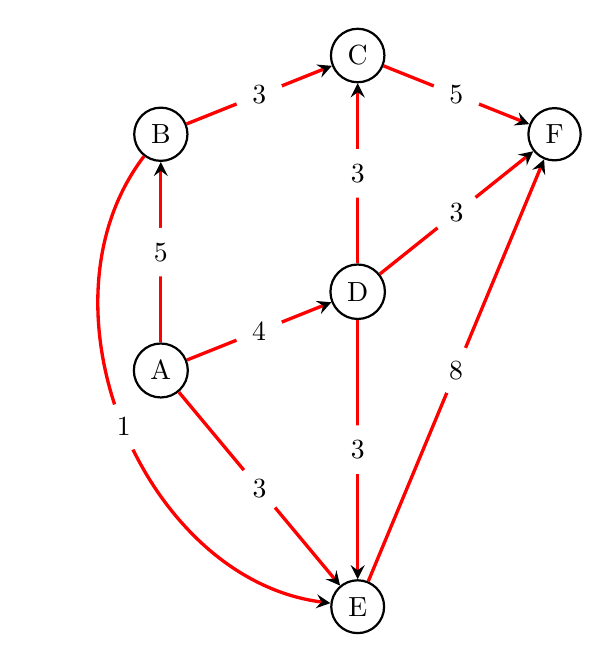
\begin{tikzpicture}
\begin{scope}[every node/.style={circle,thick,draw}]
    \node (A) at (0,0) {A};
    \node (B) at (0,3) {B};
    \node (C) at (2.5,4) {C};
    \node (D) at (2.5,1) {D};
    \node (E) at (2.5,-3) {E};
    \node (F) at (5,3) {F} ;
\end{scope}

\begin{scope}[>={stealth[black]},
              every node/.style={fill=white,circle},
              every edge/.style={draw=red,very thick}]
    \path [->] (A) edge node {$5$} (B);
    \path [->] (B) edge node {$3$} (C);
    \path [->] (A) edge node {$4$} (D);
    \path [->] (D) edge node {$3$} (C);
    \path [->] (A) edge node {$3$} (E);
    \path [->] (D) edge node {$3$} (E);
    \path [->] (D) edge node {$3$} (F);
    \path [->] (C) edge node {$5$} (F);
    \path [->] (E) edge node {$8$} (F); 
    \path [->] (B) edge[bend right=60] node {$1$} (E); 
\end{scope}
\end{tikzpicture}

\begin{tikzpicture}[
  thick,
  myrect/.style={
    draw,
    fill=myyellow,
    rectangle split,
    rectangle split parts=#1,
    rectangle split part align=left
    },
  myrect2/.style={
    draw,
    fill=myyellow,
    rectangle split,
    rectangle split draw splits=false,
    rectangle split part align=left
    },  
  mycallout/.style={
    shape=rectangle callout,
    rounded corners,
    fill=mysalmon,
    callout absolute pointer={#1},
    callout pointer width=1cm
  }  
]
\node[myrect=6,text width=1em,align=center]
  (numbers)
  {
  \strut 2
  \nodepart{two}\strut 1
  \nodepart{three}\strut 3
  \nodepart{four}\strut 3
  \nodepart{five}\strut 2
  \nodepart{six}\strut 0
  };
\end{tikzpicture}
\end{comment}
Let's consider a domain decomposition of a numerically solved partial
differential equation (PDE). Let's assume that each processor has $c = O(1)$
terms to communicate between processors. This may be a common case: in a 1D
spatial domain, simple decomposition methods do in fact yield $c = O(1))$ terms
to communicate. Let's say we have a 4-point stencil where value $u^{t+1}_x =
a(u^{t}_{x+1} + u^{t}_{x-1}) + b(u^{t}_{x})$. This produces a backward difference
method in time. When $a = r$ and $b = (1-2r)$ for $r = \kappa / h^2$, this
corresponds to the simplest finite difference approximation for the Heat
equation. When performing this update on a 1D domain, values can be updated for
time $t+1$ independently, except for the dependencies that occur at processor
boundaries. In these cases, the communication of a single value must occur
before updates take place.

Let's assume that we split our domain evenly along the spatial axis. Say we have
a domain such that
\begin{align*}
    x &\in {0, X-1} 
\end{align*}

and that we have $P$ processors in shared memory, and each processor is labeled
\begin{align*}
    p &\in {0, P-1}
\end{align*}

Processor $p$ has a chunk of of the domain with values 
\begin{align*}
    x_p     &= \{\alpha*p, \alpha*(p+1)-1\} \text{, where} \\
    \alpha  &= X / P 
\end{align*}

Given already computed values for $u^{t}_{x} ~ \forall ~ x \in X$, the values for
$u^{t+1}_{x} ~ \forall ~ x \in X$ can be computed in a data parallel manner. But
what dependencies do individual computations at time $t+1$ have on values at
time $t$? The formula provided above makes this quite apparent:
\begin{align*}
    u^{t+1}_{x} \text{ depends on } \{ u^{t}_{x-1}, u^{t}_{x}, u^{t}_{x+1} \}
    \text{.}
\end{align*}

If $x-1$, $x$, and $x+1$ are contained within $x_p$, then these values can be
accessed directly from local memory. $x \in x_p$ by definition. But, if $x =
\alpha*p$ or $x = \alpha*(p+1)$, then communication across processor boundaries
must take place, requiring communication. Communication implies synchronization,
and in order to ensure that the value has been computed, either processor $p-1$
or processor $p+1$ must tell processor $p$ that it has performed that
computation. If processors exist in separate memory spaces, the value must
actually be sent from one memory space to another. Without loss of generality,
let's say processor $p-1$ lags behind in performing its computation
indefinitely. What can processor $p$ do while it waits? It can compute values
for
\begin{align*} 
    u^{t+1}_{x_{t1}} \text{ for } x_{t1} &\in \{ \alpha*p + 1, \dots \alpha*(p+1) \} \text{,} \\
    u^{t+2}_{x_{t2}} \text{ for } x_{t2} &\in \{ \alpha*p + 2, \dots \alpha*(p+1) \} \text{,} \\
    ... \\
    u^{t+p}_{x_{t\alpha}} \text{ for } x_{t\alpha} &\in \emptyset \text{.}
\end{align*}

After $\alpha$ steps through time, processor $p$ must wait for processor $p-1$ to
finish computing its data. Likewise, waiting indefinitely for both processor
$p-1$ and $p+1$ to complete only allows for $\alpha / 2$ steps through time to be
completed. Thus, we can say that
\begin{align*}
    u^{t + i}_{\alpha*p + i-1} &\text{ depends on } p-1 \text{, and} \\
    u^{t + i}_{\alpha*(p+1)-1 - (i-1)} &\text{ depends on } p+1 \text{,} \\
                                       &\text{for } i \in \{ 1, \alpha \} \text{.}
\end{align*}

Each processor has $\alpha$ values to compute per timestep, yielding $\alpha^2$
values to compute in $\alpha$ timesteps. In this range, Processor $p$ has
$\alpha^2/4$ values that do not have dependencies on other processors,
$\alpha^2/2$ values that depend on one adjacent processor, and $p/4$ values that
depend on both adjacent processors. Every time a processor receives a value from
another processor, up to $\alpha$ new values can be computed by $p$ (in the case
that only one adjacent processor's values are needed, and $\alpha/2$ in the case
that both are).

Thus it is in the programmer's best interest to perform communication at points
in time such that each processor always has work to do: either its own work sans
dependencies, or work that relies on values from other processors. Preemptively
waiting for other processors to finish their computation results in more values
it can perform on its own, but of course results in itself being idle. But, only
asking for those values when it absolutely needs them results in a series of
coordination problems...and without the other processor realizing that it should
prioritize communicating the values it depends on, it may have to wait anyway.
Finally, constantly polling to see if adjacent processors have finished their
computation wastes time in itself.

At $t=0$, given an IVP, each processor has the full set of values $u^{0}_{x}
~ \forall ~ x \in X$. Unsurprisingly, to minimize idle processor time, computing
the values at processor boundaries serves as the best method. Interleaving from
either side, each processor can compute values at spatial points $\alpha*p$,
$\alpha*(p+1) - 1$, $\alpha*p + 1$, $\alpha*(p+1) - 2$, et cetera, for time $t =
1$. At what point in time should it attempt to compute values at time $t = 2$?
If it waits until all values at time $t = 1$ have been computed, it has
performed computations that do not depend on other processors. If later it has
to wait for values its future computations depend on, it has exhausted its own
independent computations on which it could fall back. And, it fails to supply
values that other processors need as early as it can. But, the sooner we try to
compute values at $t = 2$, the more likely that the values we need from adjacent
processors won't have been computed yet.

Stepping back from optimizing execution ordering, consider the following
strategies for dealing with synchronization.

\subsection{Preemptive Concurrency Control Scheme}
Commonly, when we synchronize values in shared memory, we perform some check to
see if the value we plan to use has been computed. We may use a spinlock, where
we check if the computing processor has relinquished its lock, and when it has,
we expect the updated value to be in place. Let's call the expected value for
the number of times we must perform this test $\Ev_\text{pre}$. Thus, to
complete a simulation with $T$ timesteps, we incur a runtime overhead of
$O(\Ev_\text{pre} T)$, because we have 2 communications per processor per
timestep; note that $\Ev_{pre}$ may depend on $N$ and $P$ and thus cannot be treated
as a constant.

In a preemptive scheme, $\Ev \geq 1$. Each processor must check to see if its
adjacent processors have computed their values the value preliminarily, and if
the test succeeds, we can use the value straightaway. If the test fails, we may
have to do some unbounded number of checks, say, if processor an adjacent
processor enters an infinite loop.

\subsection{Postemptive Concurrency Control Scheme}

In a scheme without preemptive concurrency control, if the adjacent processors
to some processor $p$ have always computed their values before $p$ accesses
them, then there could be potentially no overhead with regard to performing
tests. This precludes any verification of the shared values -- it does not
provide a mechanism for determining if the values $p$ receives from adjacent
processors have, in fact, derived from the expected computation. This leaves the
desire for a scheme that performs this verification with minimal overhead. Let's
call this overhead $\Ev_\text{post}$.

Consider two processors $p$ and $q$ that are adjacent, and processor $p$
receives value $u^{t}_{x-1}$ from $q$ while computing values for timestep $t+1$.
If values fail to be resolved before multiple timesteps have taken place on $p$,
all three values might need to be resolved. In the worst case, $p$ completes all
of its computation before $q$ has done anything. Then, $q$ will essentially, by
resolving all values in $p$, perform the entire computation of values in $p$
dependent on $q$ in serial via its resolution functions. In the best case, $q$
doesn't have to perform a single resolution, achieving nearly maximal
parallelism. To optimize this process, $p$ should perform computations that are
not dependent on $q$ while $q$ runs its resolution functions; otherwise, it
risks generating more values in need of resolution. Once all resolution has been
performed on a particular value, the reference containing the old version of
that value can be deregistered, which results in it being freed from memory, as
it no longer serves a purpose.

If the resolutions take less time, asymptotically, than the computations
themselves, the algorithm avoids the time wasted by using synchronization
schemes. The difference arises from the fact that as soon as a process computes
a value, it can either operate upon values that that process also has, or values
that another process has. If we limit computation, preemptively, to values local
to a process, the algorithm avoids latency. The algorithm should avoid
communication until absolutely necessary.

\begin{comment}
Let's assume that we split our domain evenly along both spatial axis. Say we
have a domain such that
\begin{align*}
    i &\in {0, M-1} \\
    j &\in {0, N-1}
\end{align*}

and that we have $P$ processors in shared memory, and each processor is labeled
\begin{align*}
    p &\in {0, P-1}
\end{align*}

Processor $p$ has a chunk of of the domain with values 
\begin{align*}
    i_p     &\in {\alpha*p, \alpha*(p+1)} \times {\beta*p, \beta*(p+1)} \text{, where} \\
    \alpha  &= M/\log{P} \% \log{P} \text{ and} \\
    \beta   &= N/\log{P} /  \log{P} \text{.}
\end{align*}

\begin{verbatim}
compute in shared memory all values for p_r
determine set of values to share: could be 1...s rows
serialize; mpi_isend start
mpi_irecv start; deserialize (should be free)
for each node that uses ghost node data:
compute f(data_local, data_sent)
\end{verbatim}
\end{comment}

